\renewcommand{\theequation}{\theenumi}
\begin{enumerate}[label=\arabic*.,ref=\thesubsection.\theenumi]
\item What does the equation 
\begin{align}
\vec{x}^T\myvec{1 & 0\\0 & -1}\vec{x}-\myvec{4 & 6}\vec{x}-6=0
\end{align}
become when the origin is moved to the point $\myvec{2\\-3}$?
\\
\solution
Comparing the given equation with the form:
\begin{align}
\label{eq:solutions/3/4/1/eq:conic_quad_form}
\vec{x}^T\vec{V}\vec{x}+2\vec{u}^T\vec{x}+f=0
\end{align}
We get:
\begin{align}
\vec{x}^T\myvec{1 & 0\\0 & -1}\vec{x}+2\myvec{-2 & -3}\vec{x}-6=0 \label{eq:solutions/3/4/1/2.0.2}
\intertext{where,}
\vec{V}=\myvec{1 & 0 \\0 & -1}\label{eq:solutions/3/4/1/eq:2.0.3}\\
\vec{u}=\myvec{-2 \\ -3}\label{eq:solutions/3/4/1/eq:2.0.4}\\
f=-6\label{eq:solutions/3/4/1/eq:2.0.5}
\end{align}
Here, $ \mydet{\vec{V}}=-1$. Since $ \mydet{\vec{V}}<0$ the given equation represents a hyperbola with center:
\begin{align}
\vec{c}&=-\vec{V}^{-1}\vec{u}=\myvec{2\\-3}
\end{align}

The characteristic equation of $\vec{V}$ is:
\begin{align}
\mydet{V-\lambda\vec{I}} = 0\\
\mydet{1-\lambda & 0 \\ 0 & -1-\lambda} = 0\\
\implies \lambda^2 -1 = 0
\label{eq:solutions/3/4/1/eq:asymptotes_char}\\
\lambda_{1}= 1,
\lambda_{2}= -1
\end{align}
Finding the eigen vector matrix $\vec{P}$ such that $\vec{P}^T=\vec{P}^{-1}$.      For $\lambda_1=1$

\begin{align}
    (\vec{V}-\lambda_1 \vec{I})\vec{p}
    _1=0\\
    \myvec{0 & 0 \\0 &-2 }\vec{p}_1=0 \\
    \implies \vec{p}_1=\myvec{1 \\ 0} \\
%    \text{[Choosing Orthonormal eigen vectors]} \nonumber
\end{align}
For $\lambda_2=-1$
\begin{align}
    (\vec{V}-\lambda_2 \vec{I})\vec{p}_2=0\\
    \myvec{2 & 0 \\0 &0 }\vec{p}_2=0 \\
    \implies \vec{p}_2=\myvec{0 \\ 1} \\
    \text{[Choosing Orthonormal eigen vectors]} \nonumber\\
    \vec{P}=\myvec{ \vec{p}_1& \vec{p}_2}=\myvec{1&0 \\0& 1}
\end{align}

By affine transformation $\vec{x} = \vec{P}\vec{y}+\vec{c} $,  Equation \eqref{eq:solutions/3/4/1/eq:conic_quad_form} can be written in the form:
\begin{align} 
\vec{y}^T\vec{D}\vec{y} =  \vec{u}^T\vec{V}^{-1}\vec{u} -f \\
\intertext{where,}
\vec{D} = \myvec{\lambda_1 & 0\\ 0 & \lambda_2},
\label{eq:solutions/3/4/1/eq:quad_form_hyper}
\end{align}
Thus, we can write:
\begin{align}
    \lambda_1y_1^2 -\brak{-\lambda_2}y_1^2 = \vec{u}^T\vec{V}^{-1}\vec{u} -f \label{eq:solutions/3/4/1/eq:2.0.17}
\end{align}
The equation \eqref{eq:solutions/3/4/1/eq:2.0.17} represents a modified hyperbola, The equation of the asymptotes for \eqref{eq:solutions/3/4/1/eq:2.0.17} is:
\begin{align} 
\myvec{\sqrt{\abs{\lambda_1}} & \pm \sqrt{\abs{\lambda_2}}}\vec{y} = 0 \label{eq:solutions/3/4/1/eq2.0.21}
\end{align} 
Putting the values of $\lambda_1$ and $\lambda_2$ in equation \eqref{eq:solutions/3/4/1/eq2.0.21}, we get the two asymptotes for \eqref{eq:solutions/3/4/1/eq:2.0.17}:
\begin{align} 
\myvec{1 & 1}\vec{y} = 0 \\
\myvec{1 & -1}\vec{y} = 0
\end{align} 
These are the asymptotes of our modified hyperbola. The asymptotes of our original hyberbola in equation \eqref{eq:solutions/3/4/1/2.0.2} can be obtained using:
\begin{align} 
%\label{eq:solutions/3/4/1/eq:quad_form_pair}
\myvec{\sqrt{\abs{\lambda_1}} & \pm \sqrt{\abs{\lambda_2}}}\vec{P}^T\brak{\vec{x}-\vec{c}} = 0
\label{eq:solutions/3/4/1/eq:2.0.20}
\end{align} 
Putting the values of $\lambda_1$, $\lambda_2$ and $\vec{P}$  in equation \eqref{eq:solutions/3/4/1/eq:2.0.20}, we get the equations of the asymptotes of the original hyperbola with center at $\Vec{c}$:
\begin{align} 
    \myvec{1 &-1}\myvec{1&0 \\0& 1}\brak{\vec{x}+\myvec{2 \\-3}}=0\\
    \implies \boxed{\myvec{1 &-1}\Vec{x}=5} \label{eq:solutions/3/4/1/2.0.26}\\
    \myvec{1 & 1}\myvec{1&0 \\0& 1}\brak{\vec{x}+\myvec{2 \\-3}}=0\\
     \implies \boxed{\myvec{1 &1}\Vec{x}=-1} \label{eq:solutions/3/4/1/2.0.28}
\end{align}

\begin{figure}[ht!]
    \centering
    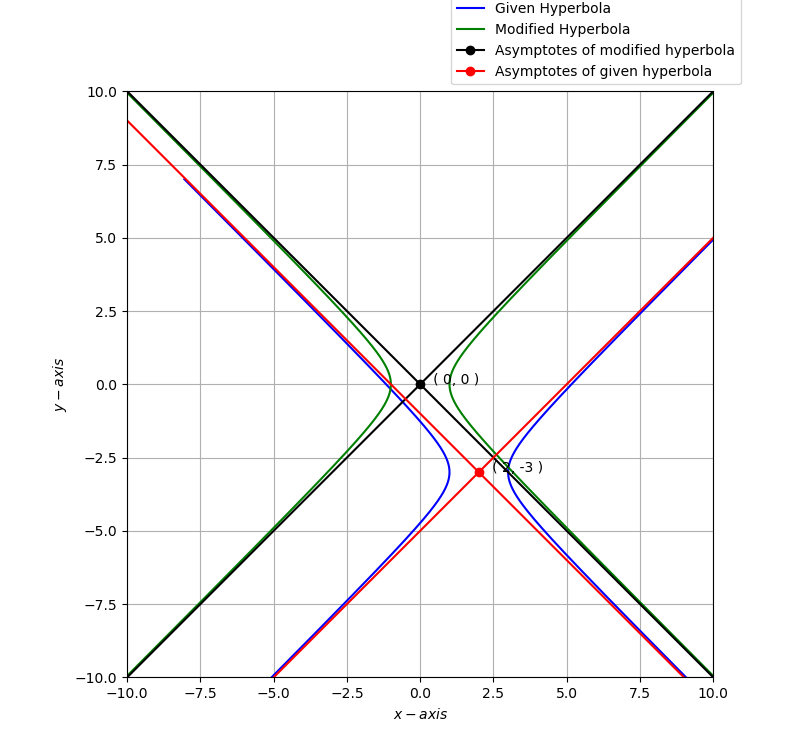
\includegraphics[width=11cm]{./solutions/3/4/1/Figure_1.png}
    \caption{Plot of the Asymtotes.}
    \label{eq:solutions/3/4/1/Plot of the Asymtotes}
\end{figure}

\item To what point must origin be shifted so that
\begin{align}\label{eq:solutions/3/4/2/eq12}
\vec{x}^T\myvec{2 & \frac{-3}{2}\\\frac{-3}{2}& 4}\vec{x}+\myvec{ 10& -19}\vec{x}+23=0
\end{align}
is transformed to 
\begin{align}\label{eq:solutions/3/4/2/eq11}
\vec{x}^T\myvec{2 & \frac{-3}{2}\\\frac{-3}{2}& 4}\vec{x}=1
\end{align}
\\
\solution
Given,
\begin{align}\label{eq:solutions/3/4/2/eq5}
\vec{x}^T\myvec{2 & \frac{-3}{2}\\\frac{-3}{2}& 4}\vec{x}+\myvec{ 10& -19}\vec{x}+23=0
\end{align}
The general second degree equation can be expressed as follows,
\begin{align}
\vec{x^T}\vec{V}\vec{x}+2\vec{u^T}\vec{x}+f=0\label{eq:solutions/3/4/2/eqmain}
\end{align}
From the given second degree equation we get,
\begin{align}
\vec{V} &= \myvec{2&\frac{-3}{2}\\\frac{-3}{2}&4}\\
\vec{u} &= \myvec{5\\\frac{-19}{2}}\\
f &= 23
\end{align}
Origin which is moved to the point is given by
$\vec{c}$
The above equation \eqref{eq:solutions/3/4/2/eqmain} can be modified as 
\begin{align}
(\vec{x}+\vec{c})^T\vec{V}(\vec{x}+\vec{c})+2\vec{u}^T(\vec{x}+\vec{c})+23&=0\label{eq:solutions/3/4/2/finalsub}
\end{align}
From equation \eqref{eq:solutions/3/4/2/finalsub} consider,
\begin{align}
    &\implies(\vec{x}+\vec{c})^T\vec{V}(\vec{x}+\vec{c})\\
    &\implies\vec{x}^T\vec{V}\vec{x}+\vec{c}^T\vec{V}\vec{x}+\vec{x}^T\vec{V}\vec{c}+\vec{c}^T\vec{V}\vec{c}\label{eq:solutions/3/4/2/1n}\\
    \intertext{we know that}
    &\vec{x}^T\vec{V}\vec{c}=\vec{c}^T\vec{V}\vec{x}\label{eq:solutions/3/4/2/p}
    \intertext{Substituting equation \eqref{eq:solutions/3/4/2/p} in equation \eqref{eq:solutions/3/4/2/1n}}
    &\implies\vec{x}^T\vec{V}\vec{x}+2\vec{c}^T\vec{V}\vec{x}+\vec{c}^T\vec{V}\vec{c}
%\label{eq:solutions/3/4/2/eq1}
\\
    \intertext{Equation \eqref{eq:solutions/3/4/2/finalsub} is modified as}
    &\implies\vec{x}^T\vec{V}\vec{x}+2\vec{c}^T\vec{V}\vec{x}+\vec{c}^T\vec{V}\vec{c}+2\vec{u}^T\vec{x}2\vec{u}^T\vec{c}+23=0
\end{align}
Equating \eqref{eq:solutions/3/4/2/finalsub} and  \eqref{eq:solutions/3/4/2/eq11}:
\begin{equation}\label{eq:solutions/3/4/2/eq1}
 \implies\vec{x}^T\vec{V}\vec{x}+2\vec{c}^T\vec{V}\vec{x}+\vec{c}^T\vec{V}\vec{c}+2\vec{u}^T\vec{x}2\vec{u}^T\vec{c}+23=
    \vec{x}^T\vec{V}\vec{x}-1
\end{equation}
From above equation \eqref{eq:solutions/3/4/2/eq1} we have,
\begin{align}\label{eq:solutions/3/4/2/eq2}
2\vec{c}^T\vec{V}\vec{x}+2\vec{u}^T\vec{x}=0
\end{align}
and
\begin{align}
2\vec{u}^T\vec{x}+\vec{v}^T\vec{c}=-22
\end{align}
From \eqref{eq:solutions/3/4/2/eq2}
\begin{align}
\vec{c}^T\vec{V}\vec{x}= -\vec{u}^T\vec{x}\\
\vec{c}^T\vec{V}= -\vec{u}^T\\
\vec{c}^T= -\vec{V}^{-1}\vec{u}^T \label{eq:solutions/3/4/2/eq45}
\end{align}
 Adjoining  $\vec V$ with identity matrix to compute inverse:
\begin{align}
\myvec{
2 &  \frac{-3}{2} &1 &0\\
 \frac{-3}{2} &4 & 0&1
}
  \xleftrightarrow[]{R_1 \leftarrow  \frac{1}{2}R_1}
\myvec{
1& \frac{-3}{4}&  \frac{1}{2}  &0\\
 \frac{-3}{2} &4 & 0 &1
}
\end{align}
\begin{align}
\myvec{
1& \frac{-3}{4}&  \frac{1}{2}  &0\\
 \frac{-3}{2} &4 & 0 &1
}
  \xleftrightarrow[]{R_2 \leftarrow R_2+\frac{3}{2} R_1}
\myvec{
1& \frac{-3}{4}& \frac{1}{2} &0\\
0 & \frac{23}{8} & \frac{3}{4} & 1}
\end{align}
\begin{align}
\myvec{
1& \frac{-3}{4}& \frac{1}{2} &0\\
0 & \frac{23}{8} & \frac{3}{4} & 1}
  \xleftrightarrow[]{R_2 \leftarrow\frac{8}{23}  R_2}
\myvec{
1& \frac{-3}{4}& \frac{1}{2} &0\\
0 & 1 & \frac{6}{23} &\frac{8}{23} }
\end{align}
\begin{align}
\myvec{
1& \frac{-3}{4}& \frac{1}{2} &0\\
0 & 1 & \frac{6}{23} &\frac{8}{23} }
  \xleftrightarrow[]{R_1 \leftarrow R_1+\frac{3}{4}R_2}
\myvec{
1& 0& \frac{16}{23} &\frac{6}{23}\\
0 & 1 & \frac{6}{23} &\frac{8}{23} }
\end{align}
\begin{align}
\vec V^{-1}=
\myvec{
\frac{16}{23} & \frac{6}{23}\\
\frac{6}{23}&\frac{8}{23}}
\end{align}
From \eqref{eq:solutions/3/4/2/eq45}
\begin{align}
\vec{c}^T=
\myvec{
\frac{-16}{23} &\frac{-6}{23}\\
\frac{-6}{23}& \frac{-8}{23}
}
\myvec{
5 \\\frac{-19}{2}
}
\end{align}
From above we have :
\begin{align}
 \vec{c}^T=
 \myvec{
 -1\\2
 }
\end{align}
Hence,
\begin{align}
 \vec c=
\myvec{
-1 &2}
\end{align}
From \eqref{eq:solutions/3/4/2/eq12} and \eqref{eq:solutions/3/4/2/eq11} when the origin is moved to the point  $\vec {c} = \myvec{-1 &2}$  $\vec{V}$ doesn't change
\begin{align}
    \det(\vec{V})&=5.75
\end{align}
Since $\det(\vec{V})>0$ the given equation represents the ellipse.
The characteristic equation of $\vec{V}$ is obtained by evaluating the determinant 
\begin{align}
       \begin{array}{|c|}
V-\lambda\vec{I}
\end{array}&=0\\
   \begin{array}{|cc|}
2-\lambda & \frac{-3}{2} \\ \frac{-3}{2} & 4-\lambda
\end{array}&=0\\
\implies 4\lambda^2-24\lambda+23&=0\label{eq:solutions/3/4/2/eqroots}
\end{align}
The eigenvalues are the roots of equation \ref{eq:solutions/3/4/2/eqroots} is given by 
\begin{align}
    \lambda_1&=\frac{6+\sqrt{13}}{2}\label{eq:solutions/3/4/2/eqeig1}\\
    \lambda_2&=\frac{6-\sqrt{13}}{2}\label{eq:solutions/3/4/2/eqeig2}
\end{align}
Hence from above:
\begin{align}\label{eq:solutions/3/4/2/d}
    \vec{D}=
    \myvec{
    \frac{6+\sqrt{13}}{2} & 0\\
     0 &\frac{6-\sqrt{13}}{2}
    }
\end{align}
The eigenvector $\vec{p}$ is defined as 
\begin{align}
    \vec{V}\vec{p}&=\lambda\vec{p}\\
    \implies (\vec{V}-\lambda\vec{I})\vec{p}&=0\label{eq:solutions/3/4/2/eqev}
\end{align}
For $\lambda_1=\frac{6+\sqrt{13}}{2}$ ,
\begin{align}
    (\vec{V}-\lambda_1\vec{I})=\myvec{\frac{-\sqrt{13}-2}{2} & \frac{-3}{2} \\\frac{-3}{2} & \frac{-\sqrt{13}+2}{2}}
\end{align}
\begin{align}
   \myvec{\frac{-\sqrt{13}-2}{2} & \frac{-3}{2} \\\frac{-3}{2} & \frac{-\sqrt{13}+2}{2}}
    \xleftrightarrow[]{R_1 \leftarrow R_1\div\frac{-\sqrt{13}-2}{2}}
    \myvec{
    1 &\frac{-\sqrt{13}-2}{2}\\
    \frac{-3}{2} & \frac{-\sqrt{13}-2}{2}
    }
\end{align}
\begin{align}
\myvec{
    1 &\frac{-\sqrt{13}-2}{2}\\
    \frac{-3}{2} & \frac{-\sqrt{13}-2}{2}
    }
    \xleftrightarrow[]{R_2 \leftarrow R_2\frac{-3}{2}R_1}
\myvec{
    1 &\frac{-\sqrt{13}-2}{2}\\
    0 &0
    }
    \end{align}
    \begin{align}\label{eq:solutions/3/4/2/p_1}
    \vec p_1=
    \myvec{
    \frac{-\sqrt{13}+2}{2}\\1
    }
\end{align}
For $\lambda_2=\frac{6-\sqrt{13}}{2}$ ,
\begin{align}
    (\vec{V}-\lambda_1\vec{I})=\myvec{\frac{\sqrt{13}-2}{2} & \frac{-3}{2} \\\frac{-3}{2} & \frac{\sqrt{13}+2}{2}}
\end{align}
\begin{align}
   \myvec{\frac{\sqrt{13}-2}{2} & \frac{-3}{2} \\\frac{-3}{2} & \frac{\sqrt{13}+2}{2}}
    \xleftrightarrow[]{R_1 \leftarrow R_1\div\frac{\sqrt{13}-2}{2}}
    \myvec{
    1 &\frac{-\sqrt{13}-2}{2}\\
    \frac{-3}{2} & \frac{-\sqrt{13}-2}{2}
    }
\end{align}
\begin{align}
\myvec{
    1 &\frac{-\sqrt{13}-2}{2}\\
    \frac{-3}{2} & \frac{-\sqrt{13}-2}{2}
    }
    \xleftrightarrow[]{R_2 \leftarrow R_2\frac{-3}{2}R_1}
\myvec{
    1 &\frac{-\sqrt{13}-2}{2}\\
    0 &0
    }
    \end{align}
    \begin{align}\label{eq:solutions/3/4/2/p_2}
    \vec p_2=
    \myvec{
    \frac{\sqrt{13}+2}{2}\\1
    }
    \end{align}
Again,for ellipse
\begin{align}
\vec{V}&=\vec{P}\vec{D}\vec{P^{-1}}
\intertext{Where $\vec{D}$ is a diagonal matrix, we get,}
\vec{P}&=\myvec{\vec{p_1}&\vec{p_2}}\\ \implies\vec{P}&=\myvec{\frac{-\sqrt{13}+2}{3} & \frac{\sqrt{13}+2}{3} \\1 & 1}\label{eq:solutions/3/4/2/eqP}\\
\vec{D}&=
    \myvec{
    \frac{6+\sqrt{13}}{2} & 0\\
     0 &\frac{6-\sqrt{13}}{2}
    }
\end{align}
Standard ellipse can be written in the form:
\begin{align}\label{eq:solutions/3/4/2/s}
    \vec{y}^T\vec{D}\vec{y}=\vec{u}^T\vec{V}^{-1}\vec{u}-f
\end{align}
Simplifying we get:
\begin{align}\label{eq:solutions/3/4/2/s1}
\vec{u}^T\vec{V}^{-1}\vec{u}=
\myvec{
5 &\frac{-19}{2}
}
\myvec
{
\frac{16}{23} & \frac{6}{23}\\
\frac{6}{23} & \frac{8}{23}
}
\myvec{
5\\\frac{-19}{2}
}
=24
\end{align}
substituting \eqref{eq:solutions/3/4/2/s1} in \eqref{eq:solutions/3/4/2/s} we have :
\begin{align}\label{eq:solutions/3/4/2/t}
 \vec{y}^T\vec{D}\vec{y}=1  
\end{align}
To get $\vec{y}$,
\begin{align}
\vec{y}&=\vec{P}^T\vec{x}-\vec{P}^T\vec{c}\\
    \vec{y}&=\myvec{\frac{-\sqrt{13}+2}{3} & 1 \\ \frac{\sqrt{13}+2}{3} & 1}
    \vec{x}-\myvec{\frac{-\sqrt{13}+2}{3} & 1\\ \frac{\sqrt{13}+2}{3} & 1}
\end{align}
Substituting  equation \eqref{eq:solutions/3/4/2/d}, in equation \eqref{eq:solutions/3/4/2/t} 
\begin{align}
    \vec{y}^T \myvec{
    \frac{6+\sqrt{13}}{2} & 0\\
     0 &\frac{6-\sqrt{13}}{2}
    }\vec{y}=1
\end{align}
\begin{figure}[h]
    \centering
    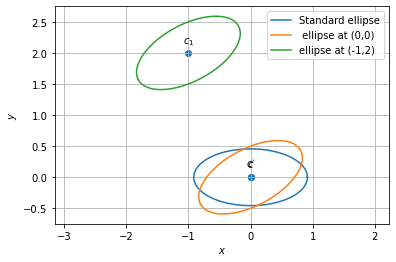
\includegraphics[width=\columnwidth]{./solutions/3/4/2/Assignment 6.png}
    \caption{Standard ellipse, Ellipse at (0,0) and  ellipse at (-1,2)}
    \label{eq:solutions/3/4/2/Fig :1}
\end{figure}

  



\item Show that the equation
\begin{align}
\vec{x}^T\vec{x}= a^2
\end{align}
remains unaltered by any rotation of the axes.
\item What does the equation
\begin{align}
\vec{x}^T\myvec{1 & \sqrt{3}\\ \sqrt{3} & -1}\vec{x} = 2a^2
\label{eq:solutions/3/4/4/eq:given}
\end{align}
become when the axes are turned through $30\degree$?
\\
\solution
The general second degree equation is expressed as follows,
\begin{align}
    \vec{x^TVx}+2\vec{u^Tx}+f=0\label{eq:solutions/3/4/4/eq:gen}
\end{align}
Comparing \eqref{eq:solutions/3/4/4/eq:given} and \eqref{eq:solutions/3/4/4/eq:gen}, we get
\begin{align}
    \vec{V}=\myvec{ 1 & \sqrt{3} \\ \sqrt{3} & -1 }\label{eq:solutions/3/4/4/eq:V}\\
    \vec{u}=\myvec{0 \\ 0}\label{eq:solutions/3/4/4/eq:u}\\
    f=-2a^2\label{eq:solutions/3/4/4/eq:f}
\end{align}
Now we find
\begin{align}
    \mydet{\vec{V}}=\mydet{1 & \sqrt{3} \\ \sqrt{3} & -1}\\
    \implies\mydet{\vec{V}}=-4\\
    \implies\mydet{\vec{V}}<0
\end{align}

Therefore the given equation \eqref{eq:solutions/3/4/4/eq:given} represents  hyperbola.

Now from affine transformations,
\begin{align}
    \vec{x}=\vec{Py}+\vec{c}
\end{align}

We have to rotate the axes by $\theta=30\degree$, Then using rotation matrix.
\begin{align}
    \vec{P}=\myvec{\cos\theta & -\sin\theta \\ \sin\theta & \cos\theta}
\end{align}
\begin{align}
    \implies\vec{P}=\myvec{\cos30\degree & -\sin30\degree \\ \sin30\degree & \cos30\degree}\\
    \implies\vec{P}=\myvec{\frac{\sqrt{3}}{2} & -\frac{1}{2} \\ \frac{1}{2} & \frac{\sqrt{3}}{2}}\label{eq:solutions/3/4/4/eq:P}
\end{align}

From eigenvalue decomposition,
\begin{align}
    \vec{P^TVP}=\vec{D}\label{eq:solutions/3/4/4/eq:eigval}
\end{align}
\begin{align}
    \implies\vec{D}=\myvec{\frac{\sqrt{3}}{2} & \frac{1}{2} \\ -\frac{1}{2} & \frac{\sqrt{3}}{2}}\myvec{1 & \sqrt{3} \\ \sqrt{3} & -1}\myvec{\frac{\sqrt{3}}{2} & -\frac{1}{2} \\ \frac{1}{2} & \frac{\sqrt{3}}{2}}\\
    \implies\vec{D}=\myvec{2 & 0 \\ 0 & -2}=\myvec{\lambda_1 & 0 \\ 0 & \lambda_2}\label{eq:solutions/3/4/4/eq:D}
\end{align}
\begin{align}
    \vec{P}=\myvec{\vec{p_1} & \vec{p_2}}\\
    \vec{P}^T=\vec{P}^{-1}
\end{align}

The equation \eqref{eq:solutions/3/4/4/eq:gen} becomes as below due to affine transformation
\begin{align}
    \vec{y}^T\vec{Dy}=\vec{u}^T\vec{V}^{-1}\vec{u}-f\label{eq:solutions/3/4/4/eq:trans}
\end{align}
with 
\begin{align}
    \vec{c}=-\vec{V}^{-1}\vec{u}\label{eq:solutions/3/4/4/eq:ctrans}
\end{align}
\begin{figure}[ht!]
    \centering
    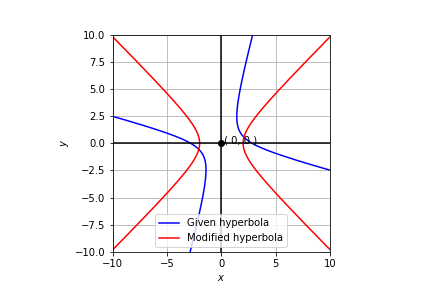
\includegraphics[width=\columnwidth]{./solutions/3/4/4/Figure}
    \caption{For $a=2$, Hyperbola rotated by $30\degree$}
    \label{eq:solutions/3/4/4/fig:figure1}
\end{figure}\\
Substitute \eqref{eq:solutions/3/4/4/eq:V},\eqref{eq:solutions/3/4/4/eq:u},\eqref{eq:solutions/3/4/4/eq:f},\eqref{eq:solutions/3/4/4/eq:D} in \eqref{eq:solutions/3/4/4/eq:trans} and \eqref{eq:solutions/3/4/4/eq:ctrans}, we get
\begin{align}
    \vec{y}^T\myvec{2 & 0 \\ 0 & -2}\vec{y}=2a^2\label{eq:solutions/3/4/4/eq:T}
\end{align}
with centre,
\begin{align}
    \vec{c}=\myvec{0 \\ 0}
\end{align}

Therefore the given equation \eqref{eq:solutions/3/4/4/eq:given} becomes \eqref{eq:solutions/3/4/4/eq:T} when the axes are turned through $30\degree$.

The plot is shown in Fig ~\ref{eq:solutions/3/4/4/fig:figure1} for a=2.

\item What does the equation
\begin{align}
\vec{x}^T\myvec{1 & -1\\-1 & 1}\vec{x}-4\sqrt{2}a\myvec{1 & 1}\vec{x}=0
\end{align}
become when the axes are turned through $45\degree$?
\\
\solution
\begin{align}
\vec{x}^T\myvec{1&-1\\-1&1}\vec{x}-4\sqrt{2}a\myvec{1&1}\vec{x}=0 \label{eq:solutions/3/4/5/eq:gen}\\
\vec{V}=\myvec{1&-1\\-1&1}\implies\mydet{\vec{V}}=0,\vec{u}=\myvec{-2\sqrt{2}a\\-2\sqrt{2}a}
\end{align}
The characteristics equation of $\vec{V}$
\begin{align}
\mydet{\lambda\vec{I}-\vec{V}}=\mydet{\lambda-1&1\\1&\lambda-1}=0\\
\implies\lambda^{2}-2\lambda=0
\end{align}
The eigen values are
\begin{align}
  \lambda{_1}=0,\lambda{_2} =2
\end{align}
 The \eqref{eq:solutions/3/4/5/eq:gen} is equation of parabola as$\lambda{_1}=0 and \mydet{\vec{V}}=0.$ 
The eigen vector $\vec{p}$ is defined as
\begin{align}
    \vec{V}\vec{p}=\lambda{\vec{p}}\\
    \implies(\lambda{\vec{I}}-\vec{V})\vec{p}=0
\end{align}
for $\lambda{_1}=0$
\begin{align}
(\lambda{_1}\vec{I}-\vec{V})= \myvec{-1&1\\1&-1}\xleftrightarrow[]{R_2\rightarrow{R_2+R_1}}\myvec{-1&1\\0&0}\\\vec{p_1}=\frac{1}{\sqrt{2}}\myvec{1\\1}
\end{align}
such that $\norm{\vec{p_1}}=1$ similarly the eigen vector for $\lambda{_2}=2$ can be find
\begin{align}
    \vec{p_2}=\frac{1}{\sqrt{2}}\myvec{-1\\1}
\end{align}
\begin{align}
\vec{P}=\myvec{\vec{p_1}&\vec{p_2}}=\frac{1}{\sqrt{2}}\myvec{1&-1\\1&1}\\
\vec{D}=\myvec{\lambda_1&0\\0&\lambda_2}=\myvec{0&0\\0&2}
\end{align}
The parabola parameters are given by
\begin{align}
    f=\frac{|\eta|}{|\lambda{_2}|} ; \eta=2\vec{p_1}^T\vec{u}\\
    f= \frac{8a}{2}=4a\\
    \myvec{0 &-6\sqrt{2}a \\ 0 & 0 \\ 0 & 2}\vec{c}=\myvec{-4a\\-2\sqrt{2}a\\0\\}\\
    \vec{c}=\myvec{0\\0} where \vec{c} is vertex
\end{align}
The axes are turned around 45\degree then 
\begin{align}
    \vec{P}=\myvec{\cos\theta & -\sin\theta \\ \sin\theta & \cos\theta}\vec{x}\\
    \vec{P}=\myvec{\cos45\degree & -\sin45\degree \\ \sin45\degree & \cos45\degree}\vec{x}\\
    \vec{P} = \frac{1}{\sqrt{2}}\myvec{1&-1\\1&1}\vec{x}
\end{align}
when $\vec{P}$ passes through the \eqref{eq:solutions/3/4/5/eq:gen} we get
\begin{multline}
\begin{aligned}
\vec{x}^T\frac{1}{\sqrt{2}}\myvec{1&1\\-1&1}\myvec{1&-1\\-1&1}\frac{1}{\sqrt{2}}\myvec{1&-1\\1&1}\vec{x}\\-4\sqrt{2}a\myvec{1&1}\frac{1}{\sqrt{2}}\myvec{1&-1\\1&1}\vec{x}=0
\end{aligned}
\end{multline}
\begin{align}
    \vec{x}^T\myvec{0&0\\0&2}\vec{x}-4a\myvec{2&0}\vec{x}=0\\
    \vec{V}=\myvec{0&0\\0&2}\implies\mydet{\vec{V}}=0
\end{align}
Therefore it is parabola..
\begin{figure}[!ht]
\centering
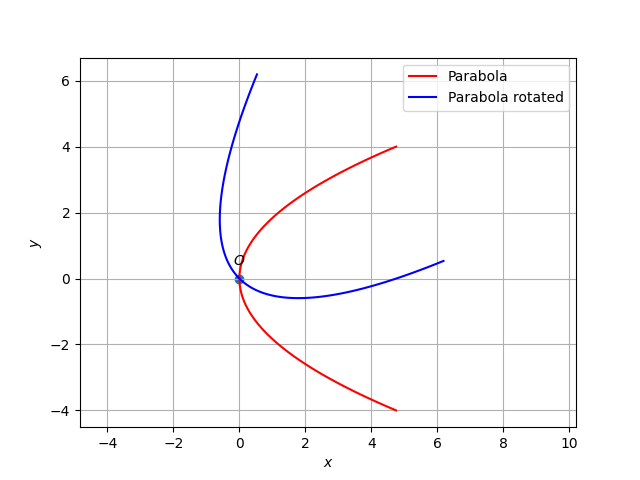
\includegraphics[width=\columnwidth]{./solutions/3/4/5/parabola.png}
\caption{ parabola with $a$ =1}
\label{eq:solutions/3/4/5/Fig}
\end{figure}

\item To what point must the origin be moved in order that the equation
\begin{align}
    \vec{x}^T\myvec{1 & 2\\2 & -2}\vec{x}+\myvec{10 & -4}\vec{x}=0 \label{eq:solutions/3/4/6/eq:q1}
\end{align}
may become
\begin{align}
    \vec{x}^T\myvec{1 & 2\\2 & -2}\vec{x}=1\label{eq:solutions/3/4/6/eq:q2}
\end{align}
and through what angle must the axes be turned in order to obtain
\begin{align}
    \vec{x}^T\myvec{p & 0\\0 & q}\vec{x}=1\label{eq:solutions/3/4/6/eq:q3}
\end{align}
\solution
The general second order equation can be expressed as follows,
\begin{align}
\vec{x^T}\vec{V}\vec{x}+2\vec{u^T}\vec{x}+f=0\label{eq:solutions/3/4/6/eq:eq1}
\end{align}
Comparing \eqref{eq:solutions/3/4/6/eq:q1} with \eqref{eq:solutions/3/4/6/eq:eq1},
\begin{align}
\vec{V} &= \myvec{1 & 2\\2 & -2}\\
\vec{u} &= \myvec{5\\ -2}\\
f &= 0
\end{align}
Let the point to which the origin is moved be $\vec{c}$\\
The above equation \eqref{eq:solutions/3/4/6/eq:eq1} can be modified as
\begin{align}
(\vec{x}+\vec{c})^T\vec{V}(\vec{x}+\vec{c})+2\vec{u}^T(\vec{x}+\vec{c})&=0\label{eq:solutions/3/4/6/eq:eq2}
\end{align}
From equation \eqref{eq:solutions/3/4/6/eq:eq2} consider,
\begin{align}
    &\implies(\vec{x}+\vec{c})^T\vec{V}(\vec{x}+\vec{c})\\
    &\implies\vec{x}^T\vec{V}\vec{x}+\vec{c}^T\vec{V}\vec{x}+\vec{x}^T\vec{V}\vec{c}+\vec{c}^T\vec{V}\vec{c}\label{eq:solutions/3/4/6/eq:eq3}\\
    &\implies\vec{x}^T\vec{V}\vec{x}+2\vec{c}^T\vec{V}\vec{x}+\vec{c}^T\vec{V}\vec{c}\label{eq:solutions/3/4/6/eq:eq4}
\end{align}
Substituting \eqref{eq:solutions/3/4/6/eq:eq4} in equation \eqref{eq:solutions/3/4/6/eq:eq2}
\begin{align}
    &\implies\vec{x}^T\vec{V}\vec{x}+2\vec{c}^T\vec{V}\vec{x}+\vec{c}^T\vec{V}\vec{c}+2\vec{u}^T(\vec{x}+\vec{c})=0 \label{eq:solutions/3/4/6/eq:eq5}
\end{align}
Comparing equations \eqref{eq:solutions/3/4/6/eq:eq5} and \eqref{eq:solutions/3/4/6/eq:q2}, we can write as,
\begin{align}
    &\implies 2\vec{c}^T\vec{V}\vec{x}+2\vec{u}^T\vec{x}=0\\
    &\implies \vec{c}^T\vec{V}= -\vec{u}^T\\
    &\implies \vec{c}= -\vec{V}^{-1}\vec{u}= -\myvec{\frac{1}{3}&\frac{1}{3}\\ \frac{1}{3}&-\frac{1}{6}}\myvec{5\\-2} \label{eq:solutions/3/4/6/eq:eq6}\\
    &\implies \boxed{\vec{c}= \myvec{-1\\-2}} \label{eq:solutions/3/4/6/eq:eq7}
\end{align}
From \eqref{eq:solutions/3/4/6/eq:eq7}, when the origin is moved to point $\vec{c}$, the equation \eqref{eq:solutions/3/4/6/eq:q1} becomes \eqref{eq:solutions/3/4/6/eq:q2}.\\
\\
From equations \eqref{eq:solutions/3/4/6/eq:q1} and \eqref{eq:solutions/3/4/6/eq:eq7}, $\vec{V}$ doesn't change
\begin{align}
    \det(\vec{V})&=-6
\end{align}
Since $\det(\vec{V})<0$ the given equation represents the hyperbola\\
\\
From equation \eqref{eq:solutions/3/4/6/eq:q2}, the equation is of the form,
\begin{align}
    \vec{x}^T\vec{V}\vec{x}+f=0
\end{align}
The matrix $\vec{V}$ can be decomposed as,
\begin{align}
    \vec{V} = \vec{P}\vec{D}\vec{P}^T \quad \vec{D}=\myvec{\lambda_1&0\\0&\lambda_2}
\end{align}
where $\lambda_1$ and $\lambda_2$ are Eigen values of $\vec{V}$, and $\vec{P}$ contains the Eigen vectors corresponding to the Eigen values $\lambda_1$ and $\lambda_2$. The affine transformation is given by,
\begin{align}
    \vec{x} = \vec{P}\vec{y}+\vec{c}
\end{align}
where, $\vec{P}$ indicates the rotation of axes and $\vec{c}$ indicates the shift of origin.\\
Eigen values of $\vec{V}$ are,
\begin{align}
   \mydet{\lambda\vec{I}-\vec{v}}=0\\
    \implies \mydet{\lambda-1&-2\\-2&\lambda+2}=0\\
    \implies \lambda^2+\lambda-6=0\\
    \implies \lambda_1=-3,\lambda_2=2\\
    \vec{D}=\myvec{-3&0\\0&2}
\end{align}
Eigen vector for $\lambda_1$=-3,
\begin{align}
    \lambda_1\vec{I}-\vec{v}=\myvec{-4&-2\\-2&-1}\xleftrightarrow[]{R_2\leftarrow R_2-\frac{R_1}{2}}\myvec{-2&-1\\0&0}\\
    \implies \vec{P_1}=\myvec{1\\-2}=\myvec{\frac{1}{\sqrt{5}}\\\frac{-2}{\sqrt{5}}}
\end{align}
Eigen vector for $\lambda_2$=2,
\begin{align}
    \lambda_1\vec{I}-\vec{v}=\myvec{1&-2\\-2&4}\xleftrightarrow[]{R_2\leftarrow R_2+2R_1}\myvec{1&-2\\0&0}\\
    \implies \vec{P_2}=\myvec{2\\1}=\myvec{\frac{2}{\sqrt{5}}\\\frac{1}{\sqrt{5}}}
\end{align}
\begin{align}
    \vec{P} = \myvec{\frac{1}{\sqrt{5}}&\frac{2}{\sqrt{5}}\\\frac{-2}{\sqrt{5}}&\frac{1}{\sqrt{5}}} \label{eq:solutions/3/4/6/eq:eq15}
\end{align}
Therefore $\vec{V}$ can be written as,
\begin{align}
    \vec{V}=\myvec{\frac{1}{\sqrt{5}}&\frac{2}{\sqrt{5}}\\\frac{-2}{\sqrt{5}}&\frac{1}{\sqrt{5}}}\myvec{-3&0\\0&2}\myvec{\frac{1}{\sqrt{5}}&\frac{-2}{\sqrt{5}}\\\frac{2}{\sqrt{5}}&\frac{1}{\sqrt{5}}}
\end{align}
Equation \eqref{eq:solutions/3/4/6/eq:q2} can be written as,
\begin{align}
    \vec{x}^T\left[\myvec{\frac{1}{\sqrt{5}}&\frac{2}{\sqrt{5}}\\\frac{-2}{\sqrt{5}}&\frac{1}{\sqrt{5}}}\myvec{-3&0\\0&2}\myvec{\frac{1}{\sqrt{5}}&\frac{-2}{\sqrt{5}}\\\frac{2}{\sqrt{5}}&\frac{1}{\sqrt{5}}}\right]\vec{x}=1\\
  \left[\myvec{\frac{1}{\sqrt{5}}&\frac{-2}{\sqrt{5}}\\\frac{2}{\sqrt{5}}&\frac{1}{\sqrt{5}}}\vec{x}\right]^T\myvec{-3&0\\0&2}\left[\myvec{\frac{1}{\sqrt{5}}&\frac{-2}{\sqrt{5}}\\\frac{2}{\sqrt{5}}&\frac{1}{\sqrt{5}}}\vec{x}\right]= 1\label{eq:solutions/3/4/6/eq:eq11}
\end{align}
Consider the rotation transformation 
\begin{align}
  \vec{x}=\vec{P}\vec{y}\\
  \implies \vec{x}=\myvec{\frac{1}{\sqrt{5}}&\frac{2}{\sqrt{5}}\\\frac{-2}{\sqrt{5}}&\frac{1}{\sqrt{5}}}\vec{y}\\
  \vec{P}^{-1}\vec{x}=\vec{P}^{-1}\vec{P}\vec{y}\\
  \implies \vec{y}= \vec{P}^{-1}\vec{x}\\
  \text{But, }\vec{P}^{-1}=\vec{P}^T\\
  \implies \vec{y}=\myvec{\frac{1}{\sqrt{5}}&\frac{-2}{\sqrt{5}}\\\frac{2}{\sqrt{5}}&\frac{1}{\sqrt{5}}}\vec{x} \label{eq:solutions/3/4/6/eq:eq12}
\end{align}
Using \eqref{eq:solutions/3/4/6/eq:eq12} in \eqref{eq:solutions/3/4/6/eq:eq11}, the equation can be rewritten as
\begin{align}
     \vec{y}^T\myvec{-3&0\\0&2}\vec{y}=1 \label{eq:solutions/3/4/6/eq:eq13}
\end{align}
Equation \eqref{eq:solutions/3/4/6/eq:eq13} is same as \eqref{eq:solutions/3/4/6/eq:q3} with $p$=-3 and $q$=2.\\
From equation \eqref{eq:solutions/3/4/6/eq:eq15}, the orthogonal matrix represents the rotation matrix in form of,
\begin{align}
    \vec{P}=\myvec{\cos\theta & \sin\theta\\ -\sin\theta& \cos\theta} \label{eq:solutions/3/4/6/eq:eq16}
\end{align}
Comparing \eqref{eq:solutions/3/4/6/eq:eq15} and \eqref{eq:solutions/3/4/6/eq:eq16},
\begin{align}
    \cos\theta = \frac{1}{\sqrt{5}}\\
    \implies \boxed{\theta = 63.43^{\circ}}
\end{align}
From equation \eqref{eq:solutions/3/4/6/eq:eq16},if the axes is turned by $\theta$ then the equation obtained would be \eqref{eq:solutions/3/4/6/eq:q3}.
\begin{figure}[h!]
	\centering
	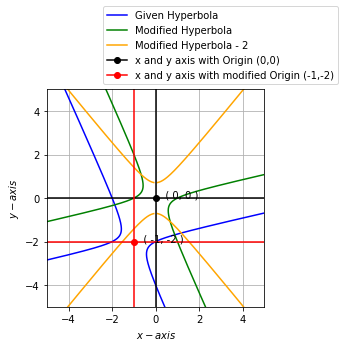
\includegraphics[width=\columnwidth]{./solutions/3/4/6/hyperbola.png}
	\caption{Hyperbola plot when origin is shifted and rotated}
	\label{eq:solutions/3/4/6/myfig}
\end{figure}

\item Through what angle must the axes be turned to reduce the equation
\begin{align}
\vec{x}^T\myvec{1 & -1\\-1 & -1}\vec{x}=1
\end{align}
to the form
\begin{align}
\vec{x}^T\myvec{0 & \frac{1}{2}\\ \frac{1}{2} & 0}\vec{x} = c
\end{align}
where $c$ is a constant.
\item 
Show that, by changing the origin, the equation
\begin{align}
2\vec{x}^T\vec{x}+\myvec{7&5}\vec{x}-13=0
\label{eq:solutions/3/4/8/eq:a0}
\end{align}
can be transformed to
\begin{align}
8\vec{x}^T\vec{x}=89
\label{eq:solutions/3/4/8/eq:a1}
\end{align}
\solution
Eq \eqref{eq:solutions/3/4/8/eq:a0} cab be written as
\begin{align}
\vec{x}^T\vec{x}+\myvec{\frac{7}{2}&\frac{5}{2}}\vec{x}-\frac{13}{2}=0\\
\implies \vec{x}^T\vec{x}+2\myvec{\frac{7}{4}&\frac{5}{4}}\vec{x}-\frac{13}{2}=0
\label{eq:solutions/3/4/8/eq:a2}
\end{align}
The above eq \eqref{eq:solutions/3/4/8/eq:a2} cab be compared with the circle equation gives as
\begin{align}
\vec{x}^T\vec{x}+2\vec{u}^T\vec{x}+f=0
\label{eq:solutions/3/4/8/eq:a3}
\end{align}
\begin{figure}[!ht]
	\centering
	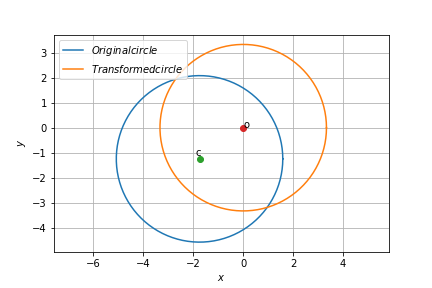
\includegraphics[width=\columnwidth]{./solutions/3/4/8/circle.png}
	\caption{Figure depicting transformation of circle}
	\label{eq:solutions/3/4/8/myfig}
\end{figure}
then
\begin{align}
\vec{u} = \myvec{\frac{7}{4}\\\frac{5}{4}}\\
\label{eq:solutions/3/4/8/eq:a4}
\implies centre, \vec{c} = \myvec{\frac{-7}{4}\\\frac{-5}{4}}\\
\norm{u}^2 - r^2 = f\\
\implies r^2 = \norm{u}^2 - f\\
\implies r^2 = \left(\frac{7}{4}\right)^2+\left(\frac{5}{4}\right)^2+\frac{13}{2}\\
\implies radius, r = \sqrt{\frac{89}{8}}
\end{align}
The eq \eqref{eq:solutions/3/4/8/eq:a1} can be written by changing the origin as
\begin{align}
\vec{(x+c)}^T\vec{(x+c)} = \frac{89}{8}\\
\implies \vec{x}^T\vec{x}+\vec{x}^T\vec{c}+\vec{c}^T\vec{x}+\vec{c}^T\vec{c} = \frac{89}{8}
\label{eq:solutions/3/4/8/eq:a5}
\end{align}
We know that
\begin{align}
\vec{x}^T\vec{c} = \vec{c}^T\vec{x}
\label{eq:solutions/3/4/8/eq:a6}
\end{align}
by substituting \eqref{eq:solutions/3/4/8/eq:a6} in \eqref{eq:solutions/3/4/8/eq:a5}
\begin{align}
\vec{x}^T\vec{x}+2\vec{c}^T\vec{x}+\vec{c}^T\vec{c} = \frac{89}{8}
\label{eq:solutions/3/4/8/eq:a7}
\end{align}
substituting the orgin of \eqref{eq:solutions/3/4/8/eq:a0} in above eq \eqref{eq:solutions/3/4/8/eq:a7}
\begin{align}
\vec{x}^T\vec{x}+2\myvec{\frac{7}{4}&\frac{5}{4}}\vec{x}+\myvec{\frac{-7}{4}&\frac{-5}{4}}\myvec{\frac{-7}{4}\\\frac{-5}{4}} = \frac{89}{8}\\
\implies \vec{x}^T\vec{x}+\myvec{\frac{7}{2}&\frac{5}{2}}\vec{x}+\frac{74}{16}-\frac{89}{8} = 0\\
\implies \vec{x}^T\vec{x}+\myvec{\frac{7}{2}&\frac{5}{2}}\vec{x}-\frac{13}{2} = 0\\
\implies 2\vec{x}^T\vec{x}+\myvec{7&5}\vec{x}-13 = 0
\end{align}
$\therefore$ It is proved that by changing the origin in \eqref{eq:solutions/3/4/8/eq:a1} we obtained \eqref{eq:solutions/3/4/8/eq:a0}.

\item Show that, by rotating the axes, the equation
\begin{align}
\vec{x}^T\myvec{3 & \frac{7}{2}\\ \frac{7}{2} & -3}\vec{x}= 1
\end{align}
can be reduced to 
\begin{align}
\sqrt{85}\vec{x}^T\myvec{1 & 0\\ 0 & -1}\vec{x}= 2
\end{align}
\item Show that, by rotating the axes, the equation
\begin{align}
\vec{x}^T\myvec{41 & 12\\ 12 & 34}\vec{x}= 75
\label{eq:solutions/3/4/10/1}
\end{align}
can be reduced to 
\begin{align}
\vec{x}^T\myvec{2 & 0\\ 0 & 1}\vec{x}= 3
\end{align}
\\
\solution
 
TThe given equation is of the form
\begin{align}
   \vec{x}^T\vec{V}\vec{x}+f=0
\end{align}
The matrix $\vec{V}$ can be decomposed as
\begin{align}
    \vec{V}=\vec{P}\vec{D}\vec{P}^T\label{eq:solutions/3/4/10/2}\\
    \text{where  }\vec{D}=\myvec{\lambda_1&0\\0&\lambda_2}
\end{align}
$\lambda_1$ and $\lambda_2$ are Eigen values of $\vec{V}$ , and
$\vec{P}$ contains the Eigen vectors corresponding to the Eigen values $\lambda_1$ and $\lambda_2$
\begin{align}
\vec{x}=\vec{P}\vec{y}+\vec{c}
\end{align}
indicates the linear transformation where $\vec{P}$ indicates the rotation of axes and $\vec{c}$ gives the shift of origin.
\begin{align}
  \vec{V}=\myvec{41&12\\12&34}\\
  det(\vec{V} )=\mydet{41&12\\12&34}>0
\end{align}
So,the given equation represents an ellipse\\
To find the Eigen values of $\vec{V}$
\begin{align}
    \mydet{\lambda\vec{I}-\vec{v}}=0\\
    \implies \mydet{\lambda-41&-12\\-12&\lambda-34}=0\\
    \implies \lambda^2-75\lambda+1250=0\\
    \implies \lambda_1=50,\lambda_2=25\\
    \vec{D}=\myvec{50&0\\0&25}
\end{align}
Finding Eigen vector $\vec{p}_1$ ,
\begin{align}
\lambda_1\vec{I}-\vec{V}= \myvec{9&-12\\-12&16}\xleftrightarrow[R_2\leftarrow R_2/4]{R_1\leftarrow R_1/3}\myvec{3&-4\\-3&4}\\
\xleftrightarrow[]{R_2\leftarrow R_1+R_2}\myvec{3&-4\\0&0}\\
\implies \vec{p_1}=\frac{1}{\sqrt{4^2+3^2}}\myvec{4\\3}=\myvec{\frac{4}{5}\\\frac{3}{5}}
\end{align}
Similarly,
\begin{align}
  \lambda_2\vec{I}-\vec{V}= \myvec{-16&-12\\-12&-9}\xleftrightarrow[R_2\leftarrow R_2/-3]{R_1\leftarrow R_1/-4}\myvec{4&3\\4&3}\\
\xleftrightarrow[]{R_2\leftarrow R_1-R_2}\myvec{4&3\\0&0}\\
\implies \vec{p_2}=\frac{1}{\sqrt{4^2+3^2}}\myvec{-3\\4}=\myvec{\frac{-3}{5}\\\frac{4}{5}}\\\text{ Therefore, } \vec{P}=\myvec{\vec{p_1}&\vec{p_2}}=\myvec{\frac{4}{5}&\frac{-3}{5}\\ \frac{3}{5}&\frac{4}{5}}
\end{align}
From \eqref{eq:solutions/3/4/10/2} $\vec{V}$ can be rewritten as
\begin{align}
    \vec{V}=\myvec{\frac{4}{5}&\frac{-3}{5}\\ \frac{3}{5}&\frac{4}{5}}\myvec{50&0\\0&25}\myvec{\frac{4}{5}&\frac{3}{5}\\ \frac{-3}{5}&\frac{4}{5}}
\end{align}
\eqref{eq:solutions/3/4/10/1} can be now rewritten as
\begin{align}
25\left[\vec{x}^T\myvec{\frac{4}{5}&\frac{-3}{5}\\ \frac{3}{5}&\frac{4}{5}}\myvec{2&0\\0&1}\myvec{\frac{4}{5}&\frac{3}{5}\\ \frac{-3}{5}&\frac{4}{5}}\vec{x}\right]=75\\
  \left[\myvec{\frac{4}{5}&\frac{3}{5}\\ \frac{-3}{5}&\frac{4}{5}}\vec{x}\right]^T\myvec{2&0\\0&1}\left[\myvec{\frac{4}{5}&\frac{3}{5}\\ \frac{-3}{5}&\frac{4}{5}}\vec{x}\right]= 3\label{eq:solutions/3/4/10/3}
\end{align}
 Consider the rotation transformation 
\begin{align}
  \vec{x}=\vec{P}\vec{y}\\
  \implies \vec{x}=\myvec{\frac{4}{5}&\frac{-3}{5}\\ \frac{3}{5}&\frac{4}{5}}\vec{y}\label{eq:solutions/3/4/10/4}\\
  \vec{P}^{-1}\vec{x}=\vec{P}^{-1}\vec{P}\vec{y}\\
  \implies \vec{y}= \vec{P}^{-1}\vec{x}\\
  \text{But, }\vec{P}^{-1}=\vec{P}^T\\
  \implies \vec{y}=\myvec{\frac{4}{5}&\frac{3}{5}\\ \frac{-3}{5}&\frac{4}{5}}\vec{x}
\end{align}

Using \eqref{eq:solutions/3/4/10/4} in \eqref{eq:solutions/3/4/10/3}, the ellipse equation can be rewritten as
\begin{align}
     \vec{y}^T\myvec{2&0\\0&1}\vec{y}=3
\end{align}
\begin{figure}[!ht]
\centering
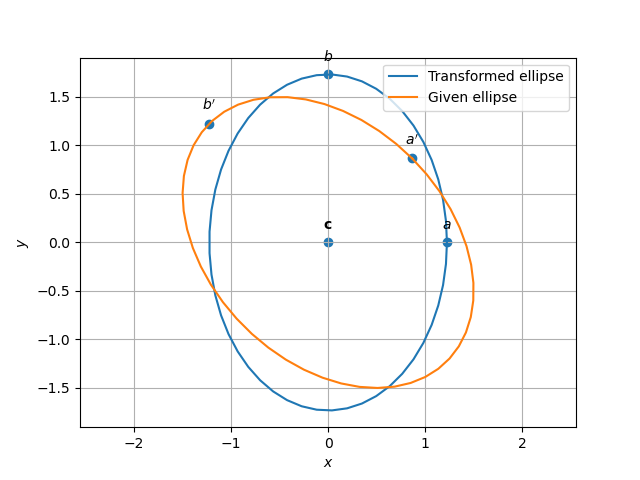
\includegraphics[width=\columnwidth]{./solutions/3/4/10/plot.png}
\caption{plot showing the original and rotated ellipse}
\label{eq:solutions/3/4/10/Fig}
\end{figure}



\item Show that, by a change of origin and the directions of the coordinate axes, the equation
\begin{align}
\vec{x}^T\myvec{5&1\\1&5}\vec{x}-\myvec{14&22}\vec{x}+27 = 0\label{eq:solutions/3/4/11/eq:0}
\end{align}
can be transformed to
\begin{align}
\vec{x}^T\myvec{3&0\\0&2}\vec{x}=1 \label{eq:solutions/3/4/11/eq:0.1}
\end{align}
or
\begin{align}
\vec{x}^T\myvec{2&0\\0&3}\vec{x}=1 \label{eq:solutions/3/4/11/eq:0.2}
\end{align}
\solution
The general second order equation can be expressed as follows,
\begin{align}
\vec{x^T}\vec{V}\vec{x}+2\vec{u^T}\vec{x}+f=0\label{eq:solutions/3/4/11/eq:1}
\end{align}
Comparing \eqref{eq:solutions/3/4/11/eq:0} with \eqref{eq:solutions/3/4/11/eq:1},
\begin{align}
\vec{V} = \myvec{5 & 1\\1 & 5}\label{eq:solutions/3/4/11/eq:2}\\
\vec{u} = \myvec{-7\\ -11}\label{eq:solutions/3/4/11/eq:3}\\
f = 27\label{eq:solutions/3/4/11/eq:4}
\end{align}
Let $\vec{c}$ be the change in the origin. The equation \eqref{eq:solutions/3/4/11/eq:1} can be modified as
\begin{align}
\vec{(x+c)^T}\vec{V}\vec{(x+c)}+2\vec{u^T}\vec{(x+c)}+f=0\label{eq:solutions/3/4/11/eq:5}
\end{align}
Considering \eqref{eq:solutions/3/4/11/eq:5}
\begin{align}
&\implies \vec{(x+c)^T}\vec{V}\vec{(x+c)}\\
&\implies \vec{x^T}\vec{V}\vec{x}+\vec{c^T}\vec{V}\vec{x}+\vec{x^T}\vec{V}\vec{c}+\vec{c^T}\vec{V}\vec{c}\label{eq:solutions/3/4/11/eq:6}
\end{align}
In the above equation
\begin{align}
\vec{c^T}\vec{V}\vec{x} = \vec{x^T}\vec{V}\vec{c}\label{eq:solutions/3/4/11/eq:7}
\end{align}
From \eqref{eq:solutions/3/4/11/eq:6} and \eqref{eq:solutions/3/4/11/eq:7} then \eqref{eq:solutions/3/4/11/eq:5} becomes
\begin{align}
\vec{x^T}\vec{V}\vec{x}+2\vec{c^T}\vec{V}\vec{x}+\vec{c^T}\vec{V}\vec{c}+2\vec{u^T}\vec{x}+2\vec{u^T}\vec{c}+f = 0\label{eq:solutions/3/4/11/eq:8}
\end{align}
Comparing \eqref{eq:solutions/3/4/11/eq:0.1} and \eqref{eq:solutions/3/4/11/eq:8}
\begin{align}
2\vec{c^T}\vec{V}\vec{P}\vec{y} + 2\vec{u^T}\vec{P}\vec{y} =0\\
\vec{c^T}\vec{V}\vec{P}\vec{y} = - \vec{u^T}\vec{P}\vec{y}\\
\vec{c} = -\vec{V^{-1}}\vec{u}\label{eq:solutions/3/4/11/eq:9}
\end{align}
Substituting \eqref{eq:solutions/3/4/11/eq:2} and \eqref{eq:solutions/3/4/11/eq:3} in \eqref{eq:solutions/3/4/11/eq:9}
\begin{align}
\vec{c}=\frac{-1}{24}\myvec{5&-1\\-1&5}\myvec{-7\\-11}=\myvec{1\\2 }\label{eq:solutions/3/4/11/eq:10}
\end{align}
Hence \eqref{eq:solutions/3/4/11/eq:8} becomes
\begin{align}
\vec{x^T}\vec{V}\vec{x}+\vec{c^T}\vec{V}\vec{c}+2\vec{u^T}\vec{c}+f = 0 \label{eq:solutions/3/4/11/eq:11}
\end{align}
Substituting \eqref{eq:solutions/3/4/11/eq:2}, \eqref{eq:solutions/3/4/11/eq:3} and \eqref{eq:solutions/3/4/11/eq:10} the above equation becomes
\begin{align}
\vec{x^T}\myvec{5&1\\1&5}\vec{x}+\myvec{1&2}\myvec{5&1\\1&5}\myvec{1\\2}+2\myvec{-7&-11}\myvec{1\\2}\\+27 = 0
\end{align}
\begin{align}
\vec{x^T}\myvec{5&1\\1&5}\vec{x}+29-58+27=0\\
\vec{x^T}\vec{V}\vec{x}-2 = 0\label{eq:solutions/3/4/11/eq:12}
\end{align}
With change in the origin to point $\vec{c}=\myvec{1\\2}$ but the $\vec{V}$ doesn't change.
\begin{align}
\mydet{\vec{V}} = \mydet{5&1\\1&5} = 24
\end{align}
As $\mydet{\vec{V}} >0$ it represents a ellipse.Hence $\vec{V}$ can be written as,
\begin{align}
\vec{V}=\vec{P}\vec{D}\vec{P^T}\label{eq:solutions/3/4/11/eq:13}
\end{align}
 The characteristic equation of $\vec{V}$ is given by
\begin{align}
\mydet{\vec{V}-\vec{I}\lambda} = 0\\
\mydet{5-\lambda & 1\\1& 5-\lambda} =0\\
\implies \lambda^2 - 10\lambda+24 = 0
\end{align}
Hence the eigen vales are,
\begin{align}
\lambda_1 = 4\\
\lambda_2 = 6
\end{align}
Hence diagonal vector is given by,
\begin{align}
\vec{D}= \myvec{\lambda_1&0\\0&\lambda_2} = \myvec{4&0\\0&6}\label{eq:solutions/3/4/11/eq:14}
\end{align}
The eigen vector $\vec{p}$ is given by
\begin{align}
    \vec{V}\vec{p}&=\lambda\vec{p}\\
    (\vec{V}-\lambda\vec{I})\vec{p}&=0
\end{align}
For $\lambda_1 = 4$  the eigenvector is,
\begin{align}
\vec{V}-\lambda_1\vec{I}= \myvec{1&1\\1&1} \xleftrightarrow[]{R_2 \leftarrow R_2-R_1}\myvec{1&1\\0&0}\\
\vec{p_1}=\myvec{\frac{1}{\sqrt{2}}\\\frac{-1}{\sqrt{2}}}
\end{align}
For $\lambda_1 = 6$  the eigenvector is,
\begin{align}
\vec{V}-\lambda_1\vec{I}= \myvec{-1&1\\1&-1} \xleftrightarrow[]{R_2 \leftarrow R_2+R_1}\myvec{-1&1\\0&0}\\
\vec{p_1}=\myvec{\frac{1}{\sqrt{2}}\\\frac{1}{\sqrt{2}}}
\end{align}
Hence,
\begin{align}
\vec{P} =\myvec{\vec{p_1}&\vec{p_2}} = \myvec{\frac{1}{\sqrt{2}}&\frac{1}{\sqrt{2}}\\\frac{-1}{\sqrt{2}}&\frac{1}{\sqrt{2}}} \label{eq:solutions/3/4/11/eq:15}
\end{align}
Substituting \eqref{eq:solutions/3/4/11/eq:14} and \eqref{eq:solutions/3/4/11/eq:15} in \eqref{eq:solutions/3/4/11/eq:13}
\begin{align}
\vec{V}= \myvec{\frac{1}{\sqrt{2}}&\frac{1}{\sqrt{2}}\\\frac{-1}{\sqrt{2}}&\frac{1}{\sqrt{2}}}\myvec{4&0\\0&6}\myvec{\frac{1}{\sqrt{2}}&\frac{-1}{\sqrt{2}}\\\frac{1}{\sqrt{2}}&\frac{1}{\sqrt{2}}}\label{eq:solutions/3/4/11/eq:16}
\end{align}
Hence substituting \eqref{eq:solutions/3/4/11/eq:16} in \eqref{eq:solutions/3/4/11/eq:12}
\begin{align}
\vec{x^T}\myvec{\frac{1}{\sqrt{2}}&\frac{1}{\sqrt{2}}\\\frac{-1}{\sqrt{2}}&\frac{1}{\sqrt{2}}}\myvec{4&0\\0&6}\myvec{\frac{1}{\sqrt{2}}&\frac{-1}{\sqrt{2}}\\\frac{1}{\sqrt{2}}&\frac{1}{\sqrt{2}}}\vec{x}=2\\
\vec{y^T}\myvec{4&0\\0&6}\vec{y}=2\\
\vec{y^T}\myvec{2&0\\0&3}\vec{y}=1\label{eq:solutions/3/4/11/eq:17}
\end{align}
where $\vec{y}$ is given by Affine transformation
\begin{align}
\vec{x}=\vec{P}\vec{y} \\
\vec{y}=\vec{P^T}\vec{x} \label{eq:solutions/3/4/11/eq:22}
\end{align}
The rotation matrix $\vec{P}$ can be given by,
\begin{align}
\vec{P}=\myvec{\cos{\theta}&\sin{\theta}\\-\sin{\theta}&\cos{\theta}}\label{eq:solutions/3/4/11/eq:18}
\end{align}
Comparing \eqref{eq:solutions/3/4/11/eq:15} and \eqref{eq:solutions/3/4/11/eq:18}
\begin{align}
\cos{\theta} = \frac{1}{\sqrt{2}}\\
\theta = \frac{\pi}{4} 
\end{align}
But given the direction of coordinate axes changes so,
\begin{align}
\theta = \pi +\frac{\pi}{4}\label{eq:solutions/3/4/11/eq:19}
\end{align}
Subtituting \eqref{eq:solutions/3/4/11/eq:19} in \eqref{eq:solutions/3/4/11/eq:18} we get 
\begin{align}
\vec{P}=\myvec{\cos{\brak{\pi +\frac{\pi}{4}}} & \sin{\brak{\pi +\frac{\pi}{4}}}\\-\sin{\brak{\pi +\frac{\pi}{4}}}&\cos{\brak{\pi +\frac{\pi}{4}}}}\\
\vec{P}=\myvec{\frac{-1}{\sqrt{2}}&\frac{-1}{\sqrt{2}}\\\frac{1}{\sqrt{2}}&\frac{-1}{\sqrt{2}}}\label{eq:solutions/3/4/11/eq:20}
\end{align}
From \eqref{eq:solutions/3/4/11/eq:13} we find the diagonal matrix
\begin{align}
\vec{D}=\vec{P^T}\vec{V}\vec{P} = \myvec{\frac{-1}{\sqrt{2}}&\frac{1}{\sqrt{2}}\\\frac{-1}{\sqrt{2}}&\frac{-1}{\sqrt{2}}}\myvec{5&1\\1&5}\myvec{\frac{-1}{\sqrt{2}}&\frac{-1}{\sqrt{2}}\\\frac{1}{\sqrt{2}}&\frac{-1}{\sqrt{2}}}\\
\vec{D}=\myvec{6&0\\0&4}\label{eq:solutions/3/4/11/eq:21}
\end{align}
Hence using \eqref{eq:solutions/3/4/11/eq:20}, \eqref{eq:solutions/3/4/11/eq:21} and \eqref{eq:solutions/3/4/11/eq:13} in \eqref{eq:solutions/3/4/11/eq:12} we get.
\begin{align}
\vec{x^T}\myvec{\frac{-1}{\sqrt{2}}&\frac{-1}{\sqrt{2}}\\\frac{1}{\sqrt{2}}&\frac{-1}{\sqrt{2}}}\myvec{6&0\\0&4}\myvec{\frac{-1}{\sqrt{2}}&\frac{1}{\sqrt{2}}\\\frac{-1}{\sqrt{2}}&\frac{-1}{\sqrt{2}}}\vec{x}=2
\end{align}
using \eqref{eq:solutions/3/4/11/eq:22} the above equation becomes,
\begin{align}
\vec{y^T}\myvec{6&0\\0&4}\vec{y}=2\\
\vec{y^T}\myvec{3&0\\0&2}\vec{y}=1\label{eq:solutions/3/4/11/eq:23}
\end{align} 
Hence from \eqref{eq:solutions/3/4/11/eq:17} and \eqref{eq:solutions/3/4/11/eq:23} proved that change of origin and the directions of the coordinate axes \eqref{eq:solutions/3/4/11/eq:0} can be tranformed to \eqref{eq:solutions/3/4/11/eq:0.1} or \eqref{eq:solutions/3/4/11/eq:0.2}
\begin{figure}[!ht]
\centering
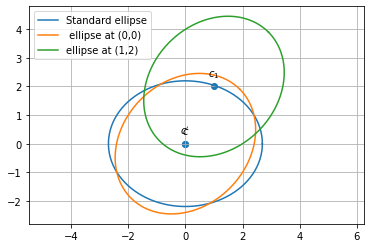
\includegraphics[width=\columnwidth]{./solutions/3/4/11/Ellipse.png}
\caption{Ellipse}
\label{eq:solutions/3/4/11/fig:Ellipse}
\end{figure}


\end{enumerate}
